\section{Problem description}
\begin{figure}
\centering
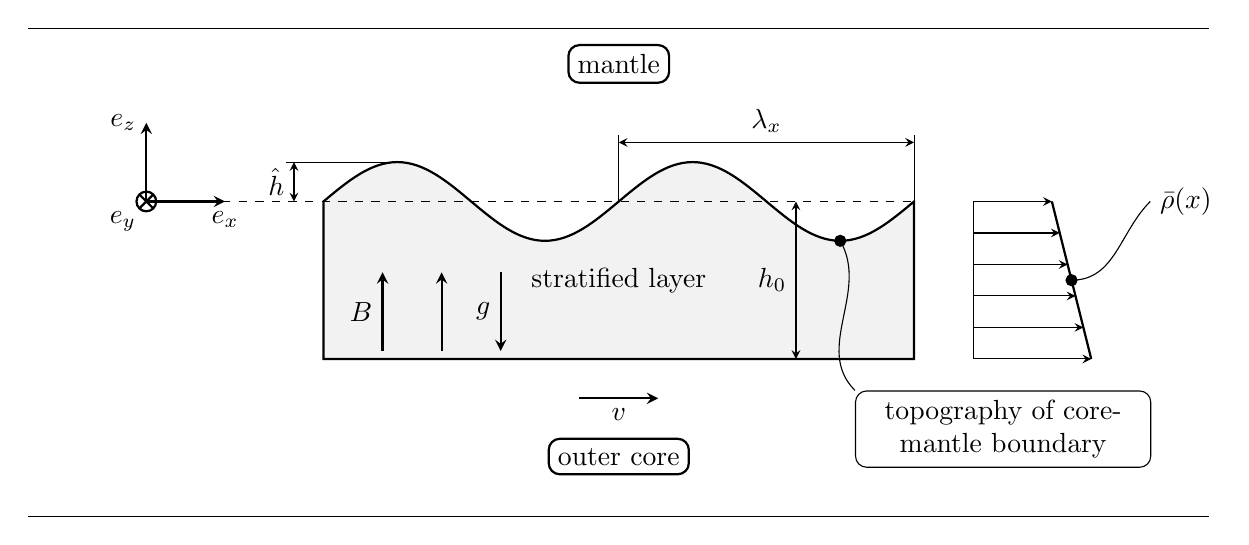
\begin{tikzpicture}[>=stealth]
	\pgfmathsetmacro\a{0.5}
	\pgfmathsetmacro\e{1.0}
	\pgfmathsetmacro\d{0.1}
	\pgfmathsetmacro\r{0.125}
	\pgfmathsetmacro\h{2.}
	\pgfmathsetmacro\b{7.5}
	\begin{scope}[shift={(-0.8*\b,\h)}]
		\draw[thick,<->] (0,\e) node[left]{$\bm{e}_z$} |- (\e,0) node[below]{$\bm{e}_x$};
		\draw[thick] (0,0) circle[radius=\r] node[below left]{$\bm{e}_y$};
		\draw[thick] (225:\r) -- (45:\r);
		\draw[thick] (135:\r) -- (-45:\r);
	\end{scope}
	% geometry
	\draw[shift={(-0.5*\b,\h)},thick,xscale=0.125*\b,fill=gray!10] (0,0) 
		sin (1,\a) cos (2,0) sin (3,-\a) cos (4,0) 
		sin (5,\a) cos (6,0) sin (7,-\a) cos (8,0) 
		-| (8,-\h) |-(0,-\h) -| cycle;
	\draw[dashed] (-0.7*\b,\h) -- (0.5*\b,\h);
	\draw[fill] (.375*\b,\h-\a) circle[radius=2pt];
	% dimensions
	\draw[<->] (0.3*\b,0) --node[midway,left]{$h_0$} (0.3*\b,\h);
	\draw (-0.375*\b,\h+\a) -- (-0.55*\b-\d,\h+\a);
	\draw[<->] (-0.55*\b,\h) --node[midway,left]{$\hat{h}$} (-0.55*\b,\h+\a);
	\draw[<->] (0,\h+1.5*\a) --node[midway,above]{$\lambda_x$} (0.5*\b,\h+1.5*\a);
	\draw (0.5*\b,\h) -- (0.5*\b,\h+1.5*\a+\d);
	\draw (0,\h) -- (0,\h+1.5*\a+\d);
	\draw (0.6*\b,0) -- (0.6*\b,\h);
	\draw[thick] (0.6*\b+1.5*\e,0) -- (0.6*\b+\e,\h);
	\foreach \i in {0,...,5}
	{
		\draw[->] (0.6*\b,\i*0.2*\h) -- (0.6*\b+1.5*\e-\i*0.1*\e,\i*0.2*\h);
	}
	% annotations
	\draw (-\b,2.1*\h) -- (\b,2.1*\h);
	\draw (-\b,-\h) -- (\b,-\h);
	\node[draw,below,thick,rounded corners] at (0,-0.5*\h) {outer core};
	\node[draw,below,thick,rounded corners] at (0,\h+4*\a) {mantle};
	\node at (0,0.5*\h) {stratified layer};
	\draw (.375*\b,\h-\a) to[in=135,out=-60] (0.4*\b,-0.2*\h) node[draw,rounded corners,text width=10em,anchor=north west,text centered]{topography of core-mantle boundary};
	\draw[fill] (0.6*\b+\e+0.25*\e,0.5*\h) circle[radius=2pt];
	\draw (0.6*\b+\e+0.25*\e,0.5*\h) to[out=0,in=225] (0.7*\b+1.5*\e,\h) node[right]{$\bar{\rho}(\bm{x})$};
	\draw[->,thick] (-0.3*\b,\d) --node[midway,left]{$\bm{\varOmega}$} (-0.3*\b,\e+\d);
	\draw[->,thick] (-0.4*\b,\d) --node[midway,left]{$\bm{B}$} (-0.4*\b,\e+\d);
	\draw[<-,thick] (-0.2*\b,\d) --node[midway,left]{$\bm{g}$} (-0.2*\b,\e+\d);
	\draw[->,thick] (-0.5*\e,-\a) --node[midway,below]{$\bm{v}$} (0.5*\e,-\a);
\end{tikzpicture}
\caption{Sketch of the stratified fluid layer at the core-mantle boundary. }
\end{figure}

The basic equations describing the problem are given by the \textsc{Navier}-\textsc{Stokes} equations using the \textsc{Boussinesq} approximation accompanied by the magnetic induction equation. The system is considered in rotating reference frame and the constant angular velocity is given by $\bm{\varOmega}=\varOmega\ez$ whose magnitude is the angular velocity of the Earth. Furthermore, the gravitational acceleration is given by $\bm{g}=-g\ez$. The corresponding dimensionless system reads:
\begin{gather}
	\nabla\cdot(\rho\bm{v})=0\,, \qquad
	\Big(\bm{v}\cdot(\nabla\otimes\bm{v})+\frac{2}{\Rossby}\bm{\varOmega}\times\bm{v}\Big)=-\nabla P+\frac{1}{\Froude^2}\rho\bm{g}+\frac{1}{\Alfven^2}\bm{B}\cdot\nabla\otimes\bm{B}\,,\\
	\nabla\cdot\bm{B}=0\,, \qquad
	\MagneticReynolds\nabla\times\left(\bm{v}\times\bm{B}\right)+\nabla^2\bm{B}=\bm{0}\,,
\end{gather}
$\Rossby$ denotes the \textsc{Rossby}, $\Froude$ the \textsc{Froude}, $\Alfven$ the \textsc{Alfv\'en} number and $\MagneticReynolds$ the magnetic \textsc{Reynolds} number. The relations of these dimensionless number to the reference quantities are given by
\begin{equation}
	\Rossby=\frac{\vref}{\varOmega\lref}\,,\quad
	\Froude=\frac{\vref}{\sqrt{\gref\lref}}\,,\quad
	\Alfven=\frac{\vref}{v_\mathrm{A}}\,,\quad 
	\MagneticReynolds=\frac{\vref\lref}{\eta}\,,
\end{equation}
where $v_\mathrm{A}=\Bref/\sqrt{\rhoref\mu}$ is the \textsc{Alfv\'en} velocity. In this problem, the reference scales are chosen as $\lref=\lambda_x$, $\rhoref=\rho_0$, $\vref=\norm{\bar{\bm{V}}}$, $\Bref=\norm{\bar{\bm{B}}}$, $\gref=\norm{\bm{g}}$. The pressure is normalized by the dynamic pressure, \ie $p_\mathrm{ref.}=\rho_0\vref^2$.

We introduce the following short-hand notations for volume and surface integrals
\begin{equation*}
	\inner{\bm A}{\bm B} = \int\limits_{\Omega} \bm A \star \bm B\, \d V \; , \quad
	\innerSurf{\bm A}{\bm B}  = \int\limits_{\Gamma} \bm A \star \bm B\, \d A \ ,
\end{equation*}
where $\bm A \star \bm B$ represents the contraction of two tensors $\bm A$ and $\bm B$ of arbitrary rank to a scalar. Furthermore, we introduce operators related to viscosity/diffusion~($\mathcal{A}$), incompressible/pressure~($\mathcal{B}$) and convection~($\mathcal{C}$).
\begin{align*}
\begin{aligned}
	\elliptic{\bm{\phi}}{\bm{\psi}}&=\inner{\nabla\bm{\phi}}{\nabla\bm{\psi}}\,, &
	\saddle{\bm{\phi}}{\psi}&=\inner{\nabla\cdot\bm{\phi}}{\psi}\,, &
	\convec{\bm{\phi}}{\bm{\psi}}{\bm{\chi}}&=\inner{\bm{\phi} \cdot (\nabla\bm{\psi})}{\bm{\chi}}\,.
\end{aligned}
\end{align*}

\section{Weak form of the hydrodynamic part}

\begin{equation}
	F(\bm{v},P,\rho)=
	\begin{bmatrix}
		-\nabla\cdot\bm{v}\\
		\bm{v}\cdot\nabla\otimes\bm{v}+\frac{2}{\Rossby}\bm{\varOmega}\times\bm{v}+\nabla P-\nu\nabla^2\bm{v}
	\end{bmatrix}
\end{equation}

\begin{equation}
	DF(\bm{v},P;\bm{\d{v}},\d{P})
	=
	\begin{bmatrix}
		-\nabla\cdot\bm{\d{v}}\\
		\bm{\d{v}}\cdot\nabla\otimes\bm{v}+\bm{v}\cdot\nabla\otimes\bm{\d{v}}+\frac{2}{\Rossby}\bm{\varOmega}\times\bm{\d{v}}+\nabla\d{P}-\nu\nabla^2\bm{v}
	\end{bmatrix}
\end{equation}

The two steps of Newton's method read
\begin{enumerate}
	\item Determine $\bm{\d{v}}^k$ and $d{P}^k$ such that
	\begin{equation}
		DF(\bm{v}^k,P^k;\bm{\d{v}}^k,\d{P}^k)=-F(\bm{v}^k,P^k)\,.
	\end{equation}
	\item Compute the updated solution according to
	\begin{equation}
		\bm{v}^{k+1}=\bm{v}^k+\bm{\d{v}}^k\,,\quad
		P^{k+1}=P^k+\d{P}^k\,.
	\end{equation}
\end{enumerate}

Weak form of the first step


If the compressibility and momentum equations are multiplied by test functions~$q$ and $\bm{w}$. After integrating the pressure by parts, the weak form reads:
\begin{gather}
-\saddle{\bm{\d{v}}^k}{q}=\saddle{\bm{v}^k}{q}\,,\label{eqn:WeakIncompressibility} \\
\begin{multlined}
	-\saddle{\bm{w}}{\d{P}^k}+\convec{\bm{\d{v}}^k}{\bm{v}}{\bm{w}}+\convec{\bm{v}}{\bm{\d{v}}^k}{\bm{w}}+\frac{2}{\Rossby}\inner{\bm{\varOmega}\times\bm{\d{v}}^k}{\bm{w}}+\nu\elliptic{\bm{\d{v}}^k}{\bm{w}}\\
	=\saddle{\bm{w}}{P^k}-\convec{\bm{v}^k}{\bm{v}^k}{\bm{w}}-\frac{2}{\Rossby}\inner{\bm{\varOmega}\times\bm{v}^k}{\bm{w}}-\nu\elliptic{\bm{v}^k}{\bm{w}}\,,
\end{multlined}\label{eqn:WeakMomentum}
\end{gather}

\section{Weak form of the continuity equation}

\begin{equation}
	S\nabla\bar{\rho}\cdot\bm{v}+\nabla\rho'\cdot\bm{v}-\nu\nabla^2\rho=0
\end{equation}
$S=\Stratification^2\Froude^2/\Rossby^2$
\begin{equation}
	F_\rho(\bm{v},\rho')=S\nabla\bar{\rho}\cdot\bm{v}+\nabla\rho'\cdot\bm{v}-\nu\nabla^2\rho'
\end{equation}

\begin{equation}
	DF_\rho(\bm{v},\rho;\bm{\d{v}},\d{\rho'})=S\nabla\bar{\rho}\cdot\bm{\d{v}}+\nabla\rho'\cdot\bm{\d{v}}+\nabla\d{\rho'}\cdot\bm{v}-\nu\nabla^2\d{\rho'}
\end{equation}

Weak form

\begin{multline}
	S\inner{\nabla\bar{\rho}\cdot\bm{\d{v}}^k}{r}+\inner{\nabla{\rho'}^k\cdot\bm{\d{v}}^k}{r}+\inner{\nabla{\d{\rho'}}^k\cdot\bm{v}^k}{r}+\nu\elliptic{{\d{\rho'}}^k}{r}=\\
	-S\inner{\nabla\bar{\rho}\cdot\bm{v}^k}{r}-\inner{\nabla{\rho'}^k\cdot\bm{v}^k}{r}-\nu\elliptic{{\rho'}^k}{r}
\end{multline}



